\section{Durchführung}
\label{sec:Durchführung}
\subsection{Effektiver Dämpfungswiderstand}
\label{sec:a}
In diesem Versuch wird die Schaltung, wie in Abb. \ref{fig:schaltung_ampli} aufgebaut.
Sie enthält einen Widerstand $R$ , Induktivität $L$ , Kapazität $C$ , ein Oszilloskop zum Messen der Amplitude und ein Generator (hier Rechteckspannung).
Es soll der kleinere der beiden festen Widerstände gewählt werden.
Nun wird auf dem Oszilloskop die Zeit eingestellt, so dass die Schwingung eines Impulses zu sehen ist. (siehe Abb. \ref{fig:aufbau_ampli})\\
Jetzt sollte eine Schwingung mit abnehmender Amplitude zu sehen sein.
Nun wird mit dem Oszilloskop die Amplitude der Spannung $U$ zum Zeitunkt $t$ gemessen.
\begin{figure}
    \centering
    \begin{subfigure}{0.48\textwidth}
        \centering
        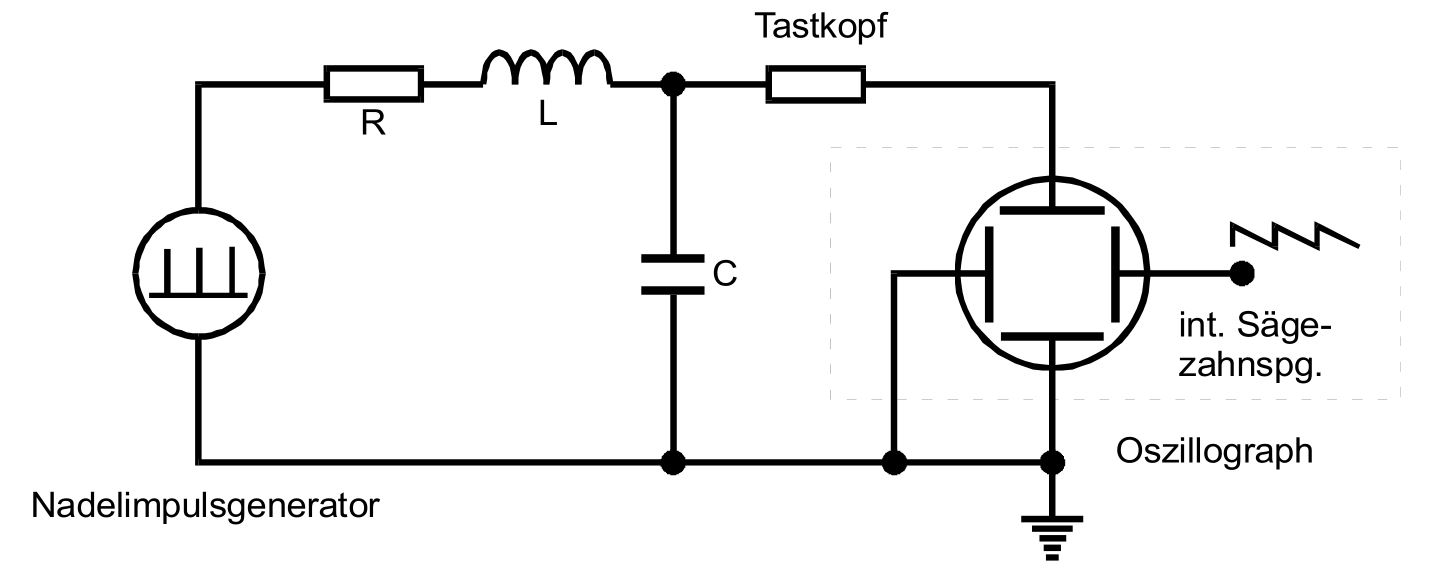
\includegraphics[height=3cm]{content/data/amplitude.jpg}
        \caption{Schaltplan eines RLC-Kreises zum Messen der Spannungsamplitude. \cite[S.294]{anleitung}}
        \label{fig:schaltung_ampli}
    \end{subfigure}
    \begin{subfigure}{0.48\textwidth}
        \centering
        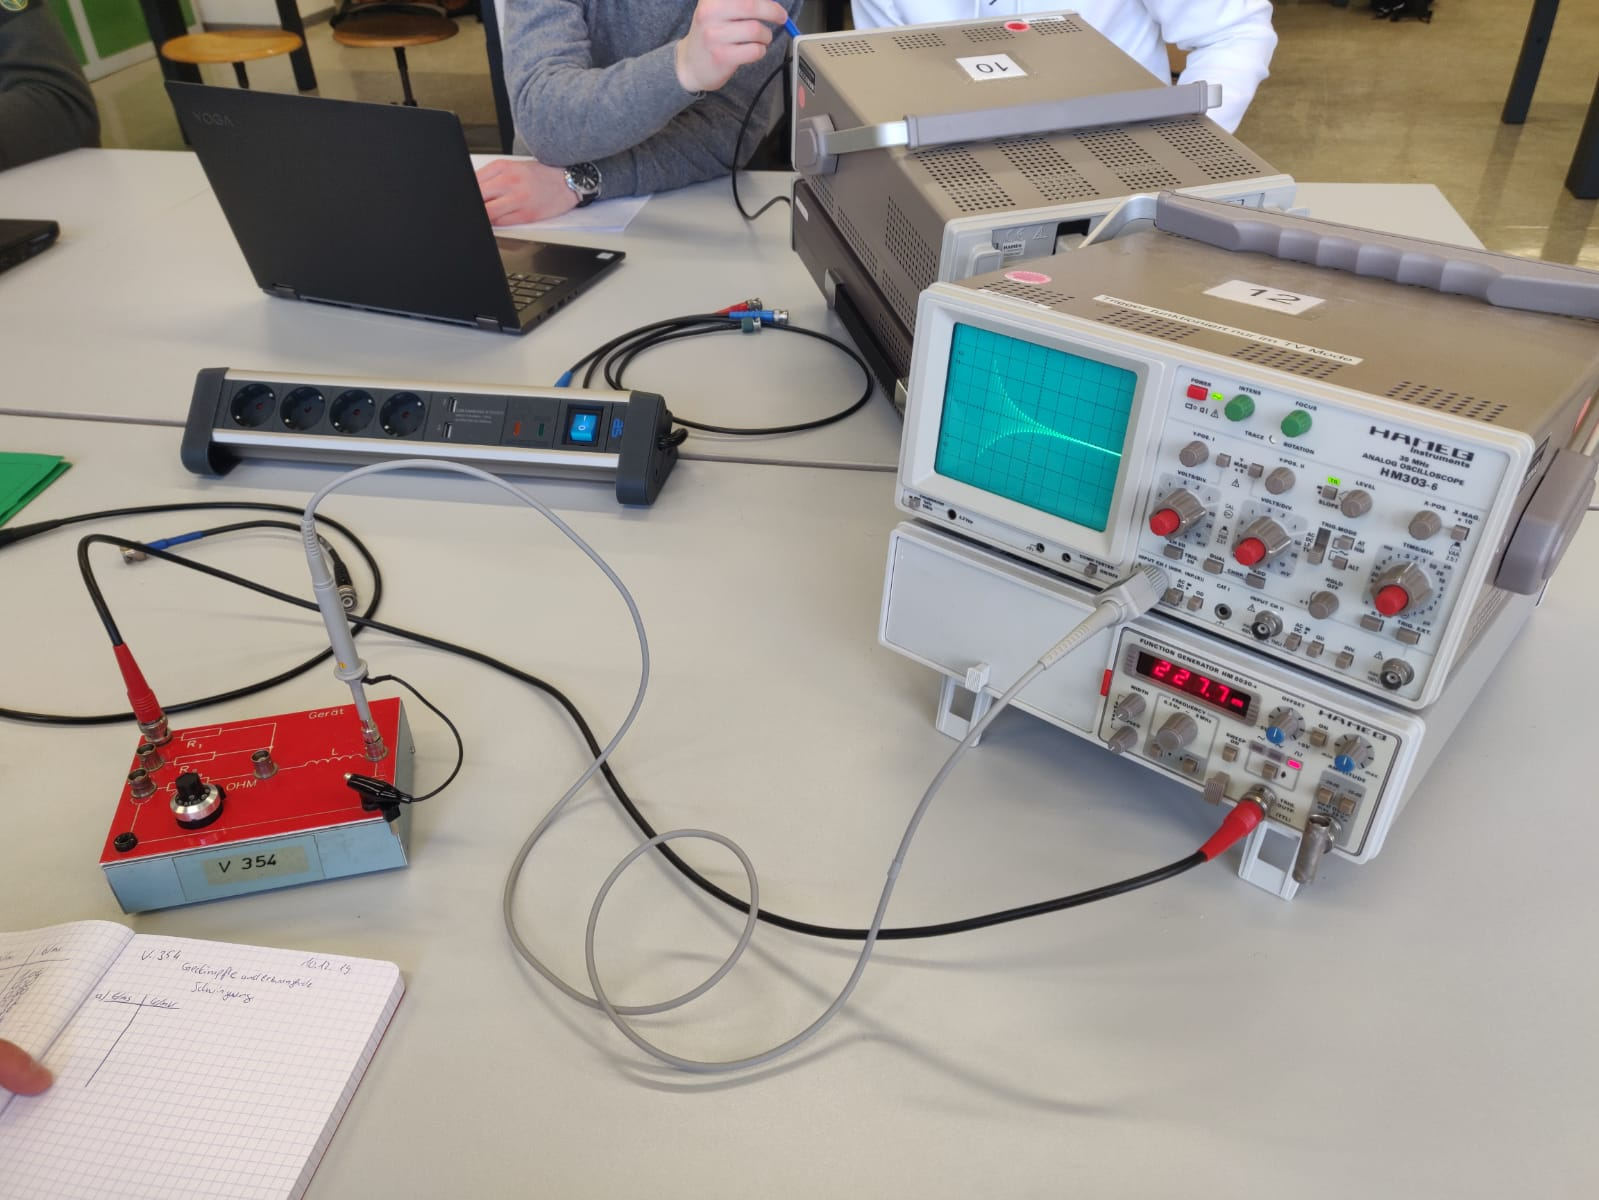
\includegraphics[height=3cm]{content/data/aufbau.jpeg}
        \caption{Aufbau des RLC Kreises mit Oszilloskop.} 
        \label{fig:aufbau_ampli}
    \end{subfigure}
    \caption{Schwingkreis mit den Bauelelementen: Kondensator mit Kapazität $C$, Spule mit Induktivität $L$, ohmscher Widerstand $R$.}
\end{figure}

\subsection{Dämpfungswiderstand bei dem aperiodischen Grenzfall}
Die Schaltung ist, wie in Abb. \ref{fig:schaltung_ampli} aufgebaut. Der in \autoref{sec:a} feste Widerstand
ist hier ein variabler Widerstand. Dieser wird zunächst auf seinen Maximalwert von \SI{10}{\mega\ohm} eingestellt.
Anschließend wird der Widerstand verringert bis ein Nulldurchgang (bzw. Überschwingen) eintritt.
Dann ist der Widerstand unter $R_\text{ap}$ gefallen und er muss wieder erhöht werden, bis der Nulldurchgang gerade verschwindet.
Dieser Wert ist dann der gesuchte $R_\text{ap}$.

\subsection{Frequenzabhängigkeit der Kondensatorspannung}
Die Schaltung wird nach Abb. \ref{fig:spannungc} aufgebaut.
Anders als zuvor wird hier eine Sinusspannung angelegt und der Generator an dem Oszilloskop angeschlossen.
Außerdem wird der größere der beiden festen Widerstände eingebaut.
Der Dämpfungswiderstand ergibt sich aus dem festen Widerstand und dem Innenwiderstand des Generators.
Nun wird die Kondensatorpannung $U_\text{c}$ und Generatorspannung $U_0$ zur Frequenz $f$ gemessen.
Es sollen etwa $15$ Messwerte im Intervall $\SI{1}{\kilo\hertz}$ bis $\SI{100}{\kilo\hertz}$ aufgenommen werden.
Hier ist $U_0$ konstant und muss daher nur einmal gemessen werden.
Bei einer bestimmten Frequenz wird ein Maximum erwartet.
Um dieses genauer darstellen zu können wird in der Nähe des Minimums in kleineren Schritten gemessen.
\begin{figure}
    \centering
    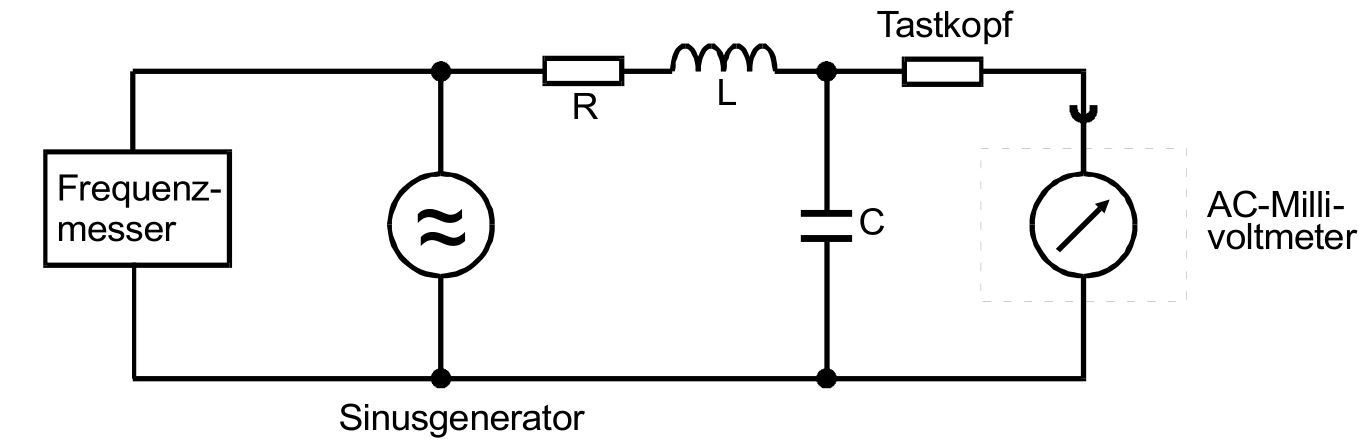
\includegraphics[width=10cm]{content/data/frequenz.jpg}
    \caption{Schaltung um frequenzabhängige Amplitude zu messen. \cite[S.295]{anleitung}}
    \label{fig:spannungc}
\end{figure}

\subsection{Frequenzabhängigkeit der Phase}
Zunächst wird die Schaltung (Abb. \ref{fig:phase}) aufgebaut.
Am Oszilloskop ist jetzt zum einen die Kondensatorspannung $U_\text{c}(t)$ und zum anderen die Spannung des Sinusgenerators $U_\text{G}(t)$ zu sehen.
Nun wird wie zuvor die Frequenz im selben Kilohertz-Bereich variiert und $15$ Messwerte aufgenommen.
Dann wird der Abstand $a$ zwischen den Nulldurchgängen der sinusförmigen Spannungen gemessen und ebenfalls die Wellenlänge $b$ notiert (siehe Abb. \ref{fig:phase_ab}).
Die Phasenverschiebung in rad ergibt sich dann aus $\frac{a}{b}2\pi$.
\begin{figure}
    \centering
    \begin{subfigure}{0.48\textwidth}
        \centering
        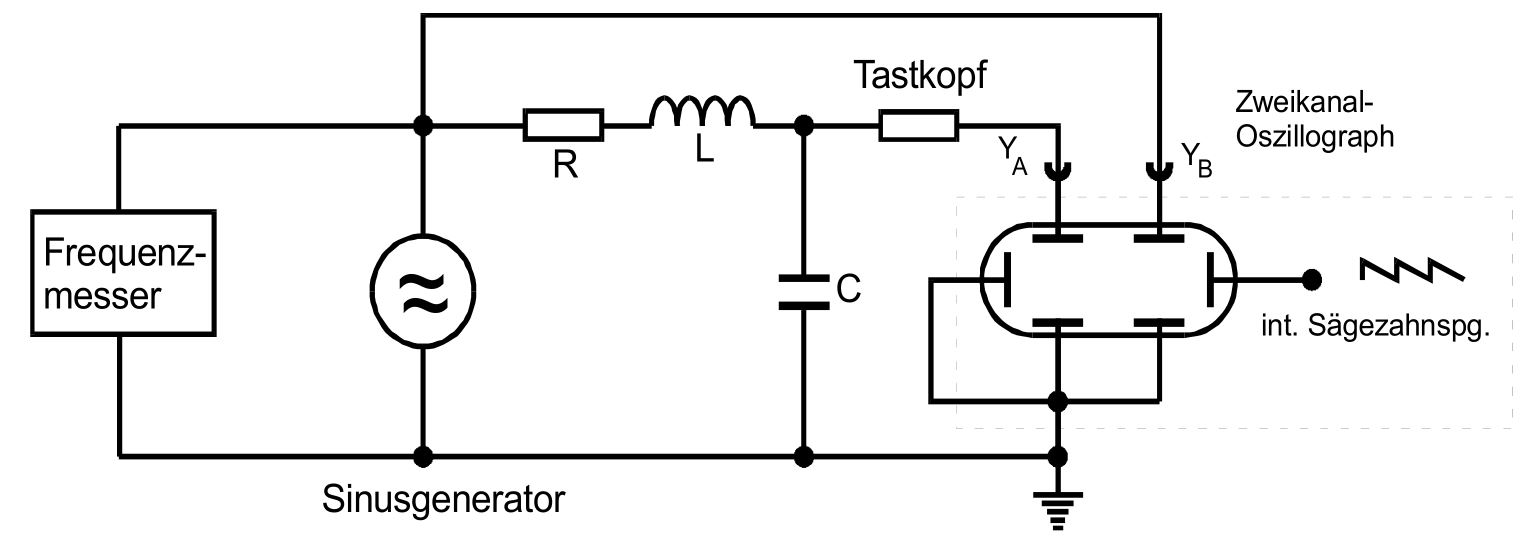
\includegraphics[height=3cm]{content/data/phase.jpg}
        \caption{Schaltplan zur Messung der Phasenverschiebung zwischen Kondensatorspannung $U_\text{c}$ und Generatorspannung $U$. \cite[S.296]{anleitung}}
        \label{fig:phase}
    \end{subfigure}
    \begin{subfigure}{0.48\textwidth}
        \centering
        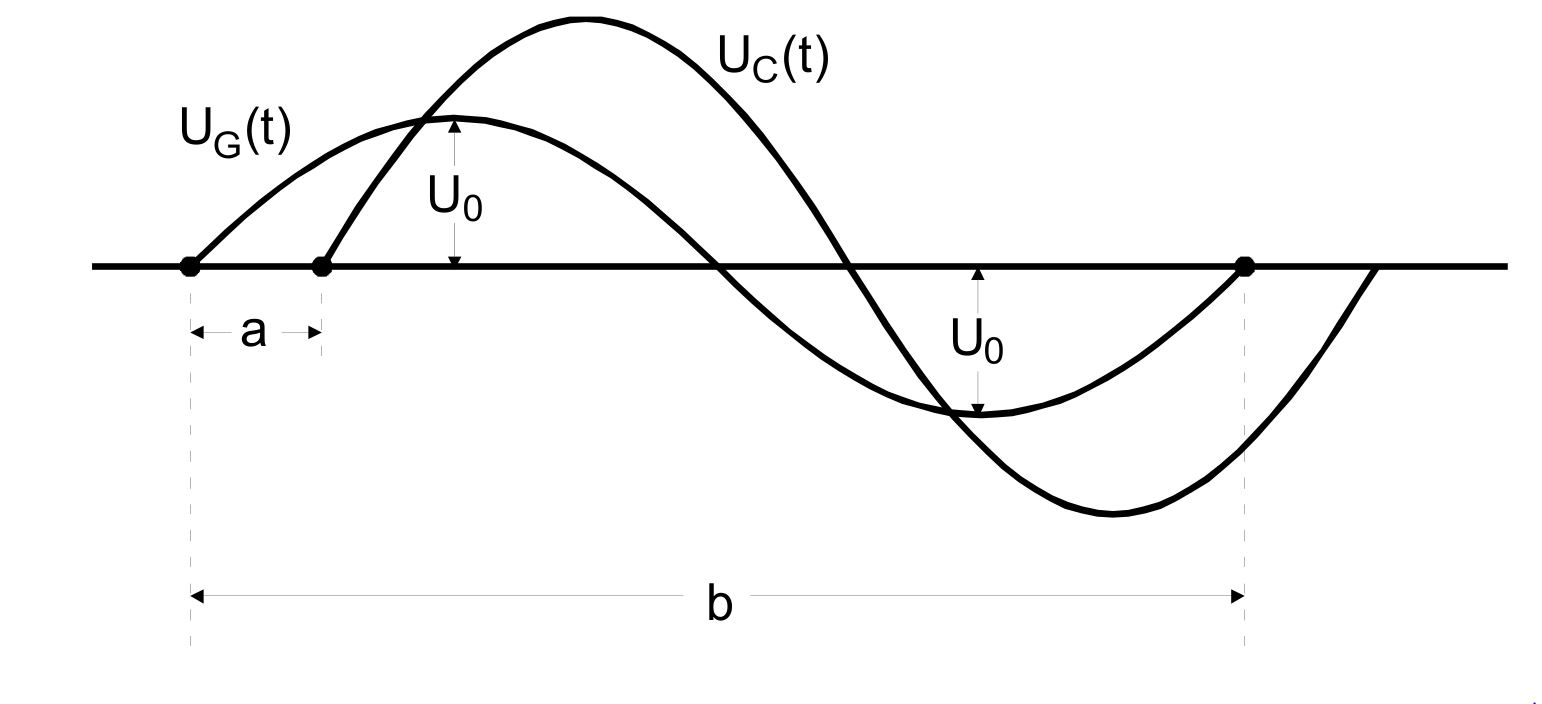
\includegraphics[height=3cm]{content/data/phase_ab.jpg}
        \caption{Definition der Längen $a$, $b$. \cite[S.282]{anleitung_rc}} 
        \label{fig:phase_ab}
    \end{subfigure}
    \caption{Erzwungene Schwingung mit Erregerfrequenz $\omega$ des Sinusgenerators.}
\end{figure}